\chapter{Controls}%
\label{ch:controls}
Control systems are responsible for computing the commands necessary for actuators to cause the trajectory of a system to go from its current state to a desired state, or for answering the question ``How do I get there?'' There are many different methods that can be used to determine the output commands, one of the more popular and widely implemented being the proportional-integral-differential (PID) controller.
Model-based controllers utilize knowledge of the physics of the system to compute appropriate output commands.
The robots in these experiments originally used PID controllers for heading control.
Later, they were tested with a model-based contoller that takes advantage of Lyapunov stability theory.
Both types of controllers described in this chapter take in state estimates from the Kalman filter of Chapter~\ref{ch:estimation} and output linear and angular velocity commands to the robots.

\section{PID}%
\label{sec:pid}
PID controllers use the current state estimate to determine the errors between the desired state and the current state.
The goal of the PID controller is to drive those errors to zero based on a number of criteria, including rise time, settling time, steady state error and overshoot.
Shown in Figure~\ref{fig:pid}, the green line is the ideal output, while the blue and purple lines are typical results.
The orange line shows what happens when a system becomes unstable.
Point $m$ represents the desired state, $m-n$ represents steady state error, point $a$ is the rise time for the blue line and point $b$ is the settling time for the blue line.

\begin{figure}[ht!]
\centering
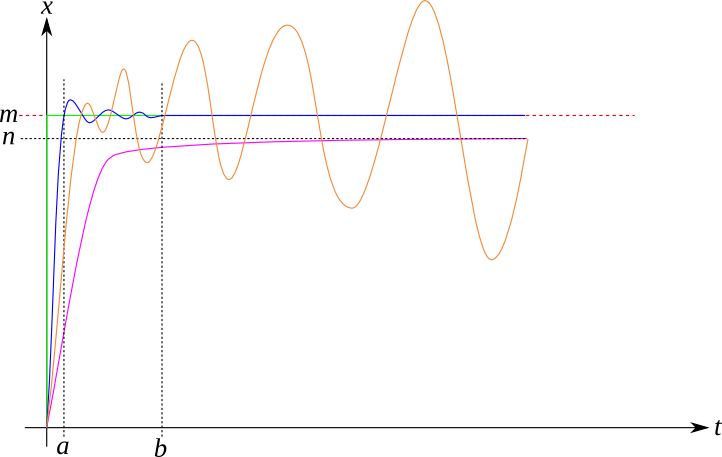
\includegraphics[width=.85\textwidth]{images/pid}
\caption{PID Controller Response}%
\label{fig:pid}
\end{figure}

The process used to compute an output command using a PID controller uses three separate errors and a gain for each of the distance and heading errors.
Looking at the PID controller for heading, the errors are
\begin{align*}
\begin{split}
E_P &= \psi_{\text{ref}_k} - \psi_k \\
E_I &= \sum_{i=0}^{k}E_{P_i}*\Delta_T \\
E_D &= \frac{\psi_k - \psi_{k-1}}{\Delta_T}
\end{split}
\end{align*}
where $\psi_{\text{ref}_k}$ is the desired heading at the current time, $\psi_k$ is the current heading estimate, $\psi_{k-1}$ is the previous heading estimate and $\Delta_T$ is the time elapsed since the last PID control calculation was performed.
The contribution of each error is then weighted by a gain to obtain the final output command, $\omega$, such that
\begin{align*}
\omega = K_P*E_P + K_I*E_I + K_D*E_D
\end{align*}
where $K_P$ is the proportional gain, $K_I$ is the integral gain and $K_D$ is the differential gain.

The only parameters available to tune PID controllers for performance are the gains.
There are some rules of thumb for tuning gains properly as described in~\cite{ZeiglerNichols42} that can work as a good starting point.
A basic knowledge of what the effects are when modifying the different gains is summarized in Table~\ref{tab:PIDGainEffects}.
The difficulty in using PID controllers for the small robots used in these experiments is that the gains must be tuned for specific operating scenarios, so that a set of gains that work well at full speed on asphalt do not work at all when the robot is driving in soft sand at any velocity.
PID controllers work best when they only have to reject a small range of disturbances, but military robots are often required to operate in environments with a large range of disturbances.

When the characteristics of a robot are changed, the PID gains must also be modified to reflect those changes.
These characteristics include mass, center of mass, treads, motors, and payloads, as these all affect the dynamics of the system.
Gain scheduling is the process of tuning a system to use a different set of gains based on the operating environment or characteristics of the robot and is very time consuming.
All these issues motivate the search for a better control system for small robots.

Table~\ref{tab:PIDGainEffects} shows how increasing the different gain values affects the performance of the controller output in terms of rise time, overshoot, settling time and steady-state error.
It can be seen that a large amount of coupling exists between the gains,  and attempting to fix one aspect of the controller output can have unintended consequences that cause other aspects to perform poorly.
This coupling is in contrast to the gains that arise for model-based controllers as seen in Section~\ref{sec:lyapunovTrajectoryConvergence}.

\begin{table}[ht!]
\caption{Effects on Controller Output of Modifying PID Gains}
\small
\centering
\begin{tabular}{@{}llllr@{}} \toprule
Parameter    & Rise Time      & Overshoot & Settling Time & Steady State Error \\ \midrule
$K_p$        & Decrease       & Increase  & Small Change  & Decrease \\
$K_i$        & Decrease       & Increase  & Increase      & Eliminate \\
$K_d$        & Small Decrease & Decrease  & Decrease      & None \\ \bottomrule
\end{tabular}%
\label{tab:PIDGainEffects}
\end{table}

\subsection{PID Implementation}
The PID controller used by SSCPAC was only for angular rate output, with the linear velocity output set to a maximum allowable velocity, and a simple ramp function used to slow the robot down as it approached a waypoint.
In conjunction with the PID controller, a simple local path planner was developed following work in~\cite{Hogg02}.
This path planner uses a carrot placed a reasonable distance in front of the robot on the path from the previous to the current waypoint, and the carrot position, rather than the waypoint position, is used to correct the heading.
When the waypoint is a large distance from the robot's current position, this causes the PID controller to move the robot onto the path faster than it would if the heading error were only based on the angle to the waypoint.
The carrot could also be extended along the path after the waypoint so that the robot would not stop at each intermediate waypoint, but would instead cut the corner on the way to the next waypoint.
One of the difficulties in using the PID controller, and a motivation for finding a different control scheme, is that as the maximum allowable linear velocity is set to larger values, the performance of the controller works poorly when the waypoints are spaced close together, as is the case when obstacles are present.
The converse is also true.
As previously mentioned, gain scheduling is a time-intensive task but it is possible that it would have provided a working solution.

\section{Model-Based Controller}%
\label{sec:lyapunov}
The motivation to find a replacement for the PID controller was primarily caused by one major shortcoming.
When the PID gains were set to work well with the robot running at full speed, performance degraded when slowing down, as is typically the case when obstacles are encountered.
Conversely, tuning the gains to work at slow speeds caused the robot to drive poorly at fast speeds.
As will be shown in Chapter~\ref{ch:results}, the model-based controller works well at varying speeds.
There are also cases where the PID controller becomes unstable and cannot converge to a goal position, while the model-based controller does not suffer from this deficiency.

An alternative control method to using classical PID controllers is to use model-based controllers based on Lyapunov stability theory.
An intuitive way to conceptualize controllers based on this stabilty theory is by thinking of them as decreasing the overall energy of a system, even when the variables involved in the control Lyapunov functions do not represent energy~\cite{Khalil02}.

The theorem for Lyapunov stability states that, for an equilibrium point $x=0$ and a domain $D\subset\mathbb{R}^n$ that contains $x=0$, and for which there is a function $V:D\to\mathbb{R}$ that is continuously differentiable and has the following properties 
\begin{align}
\label{eq:lyapunovTheorem}
\begin{split}
V(0) &= 0 \\
V(x) &> 0 \in D-\{0\} \\
\dot{V}(x) &\leq 0 \in D-\{0\}
\end{split}
\end{align}
then the equilibrium point $x=0$ is stable.
Additionally, if
\begin{align}
\label{eq:lyapunovAsymptoticStability}
\dot{V}(x) < 0 \in D - \{0\}
\end{align}
then $x=0$ is asymptotically stable.

It is not always possible to find such a control Lyapunov function $V$, but when one is found then this theorem holds and the ``energy'' of the system will always be positive and decreasing.
The ``energy'' can consist of any variables that make $V(0) = 0$ and $V(x) > 0$ and consist of a combination of the errors that are to be minimized in a system.
In that case the errors are always decreasing, since $\dot{V}(x) < 0$, and the system will reach the desired state.

Two different modes of the model-based controller were developed and tested during these experiments.
The difference between the two modes is the behavior of the robot as it approaches intermediate waypoints while navigating to its final destination.
The first mode is considered to be useful for a parking behavior where the robot stops at each waypoint, including the intermediate waypoints.
The second mode is a slightly modified version of the parking behavior, where the distance error is extended beyond each intermediate waypoint so that the robot will drive through the waypoints without stopping (although the robot often does slow down some) until it reaches its final destination.
This second mode will be referred to as the driving mode.
During the following development of the control law, the parking mode will be described fully, then extensions will build directly on top of the parking mode to describe the driving mode in Section~\ref{sec:drivingMode}.

\subsection{Error Terms for the Model-Based Controller}%
\label{sec:errorTermsMBC}
Several groups have implemented model-based controllers rooted in Lyapunov stability theory in simulation including~\cite{MicaelliLyapunov93},~\cite{Aicardi94},~\cite{Aicardi_UnicycleLyapunov95},~\cite{Rusu05RobotuxLyapunov},~\cite{Gulati08}.
Only recently have these results been applied to actual robots~\cite{KimLyapunov05},~\cite{Lapierre06},~\cite{Lapierre07},~\cite{NuchterLyapunov07}.
All of these groups describe a method for constructing a control Lyapunov function based on the kinematics of a differential-drive robot, similar to the small robots considered in these experiments, which are typically referred to as unicycle-like robots in the literature.

\begin{figure}[ht!]
\centering
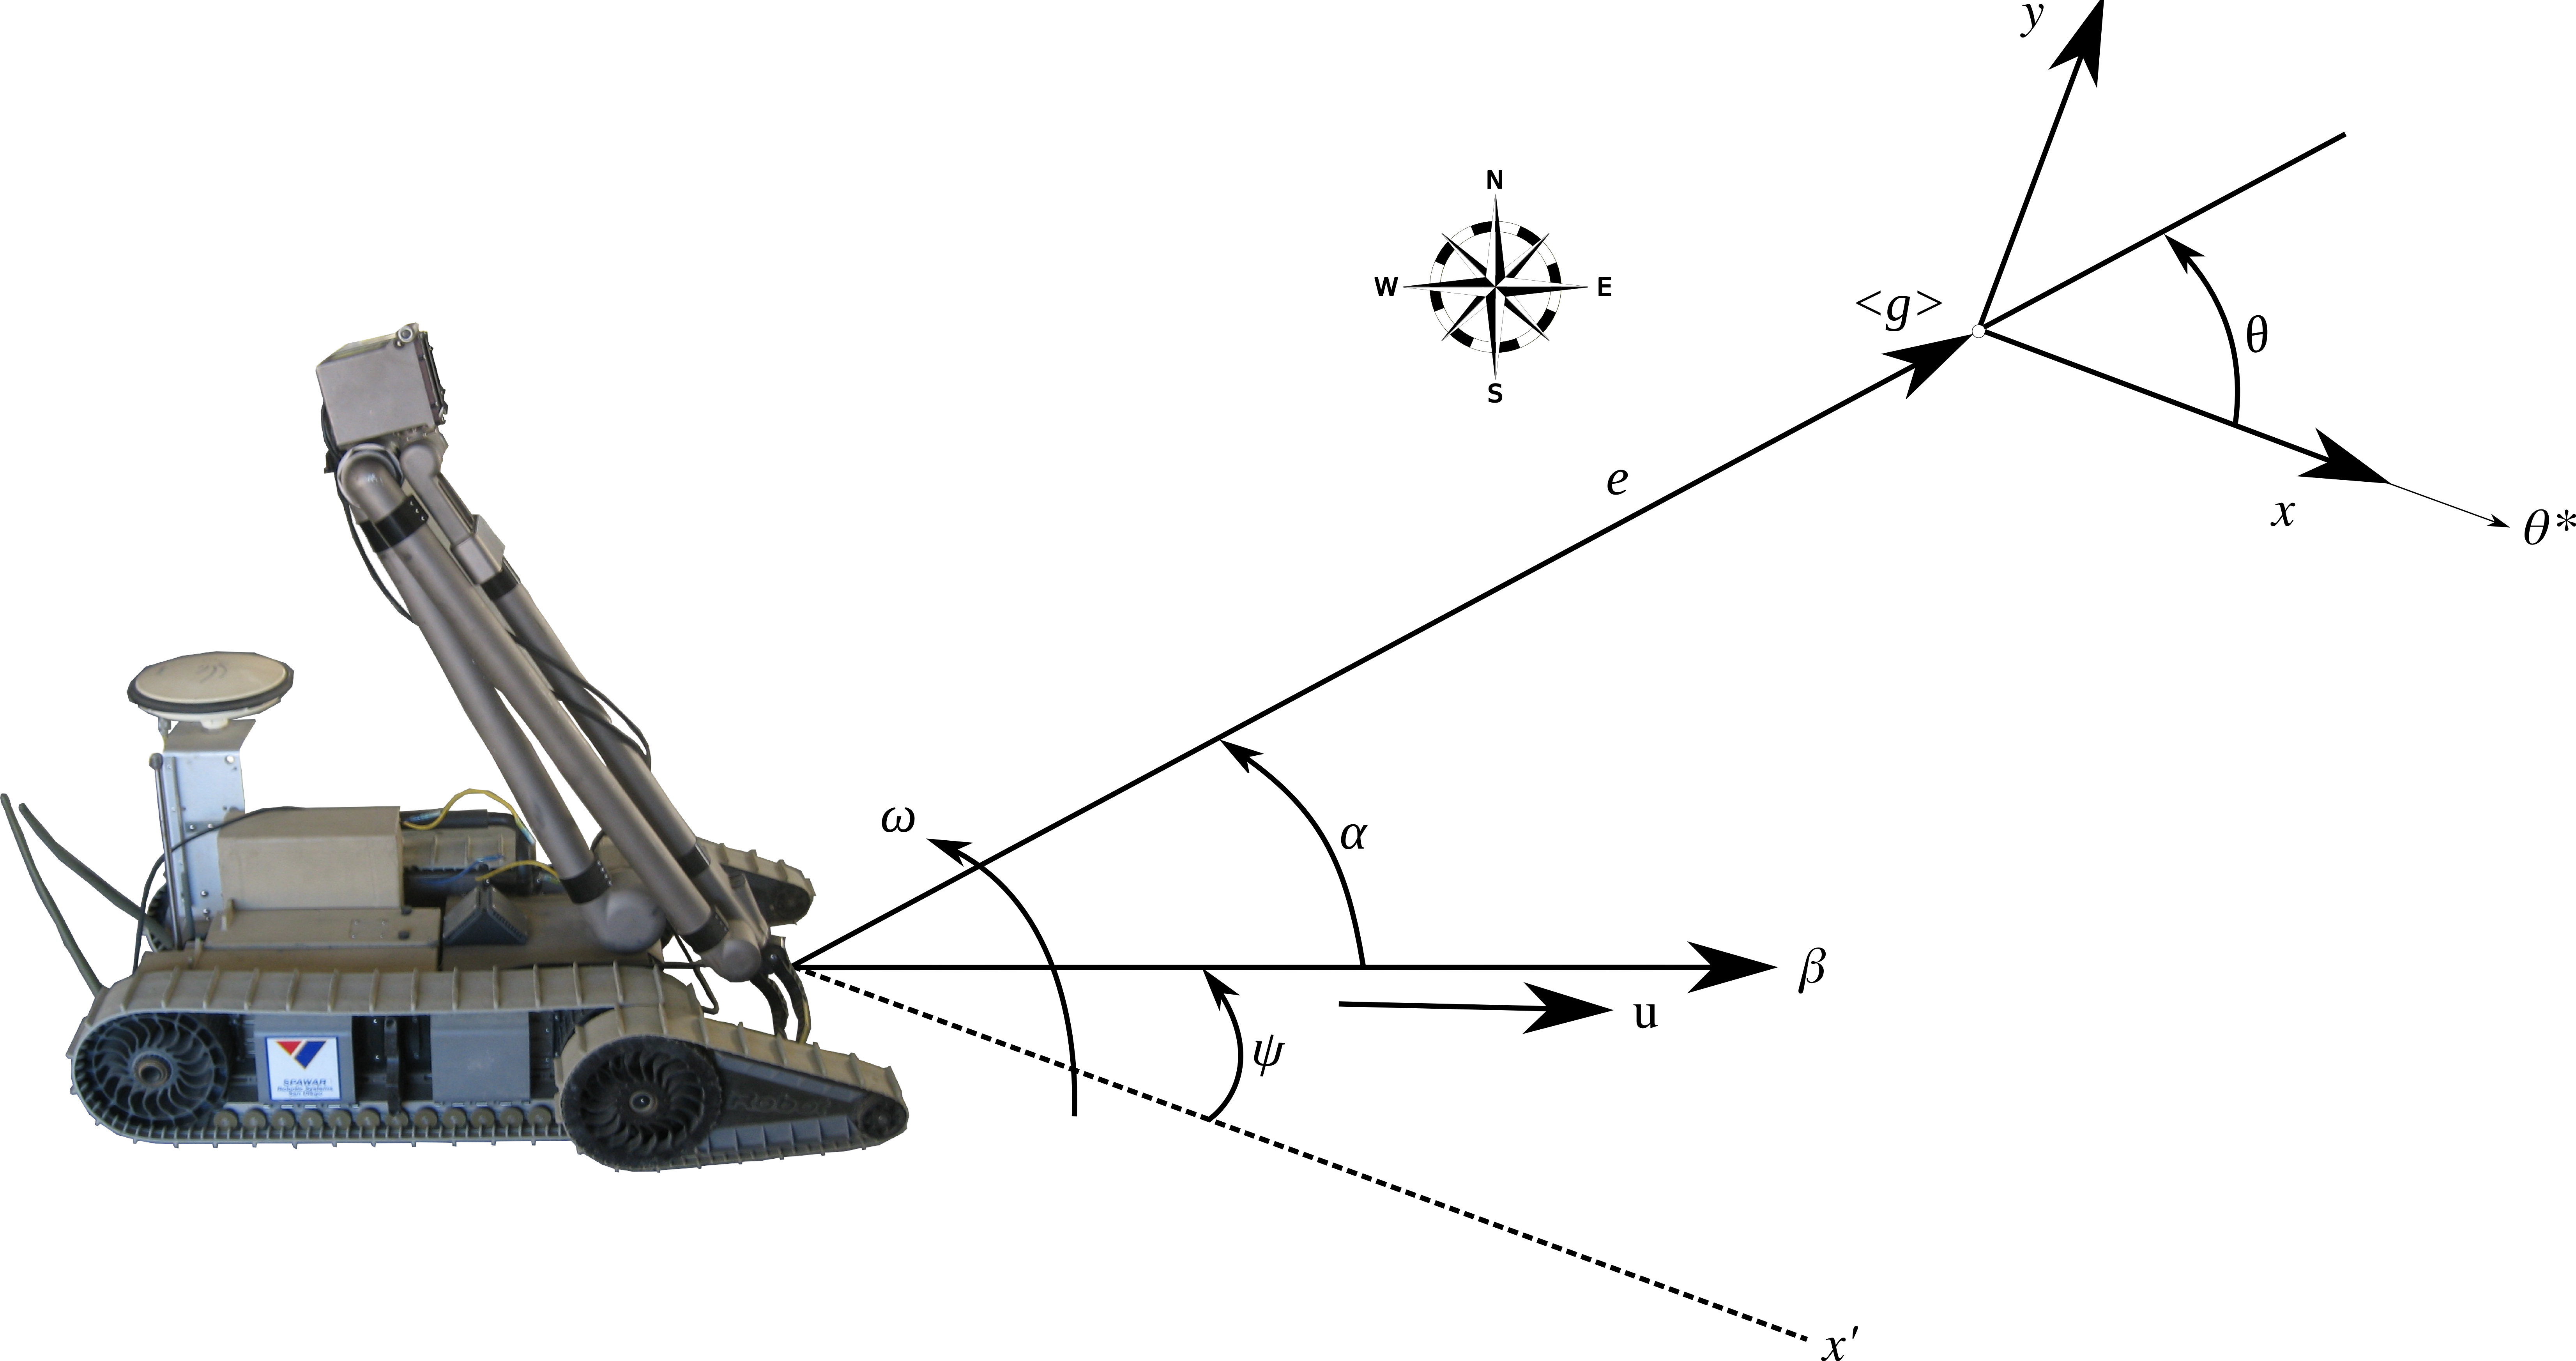
\includegraphics[width=.95\textwidth]{images/packbotlyapunov}
\caption{Packbot Coordinate System for Model Based Controller}%
\label{fig:pblyapunov}
\end{figure}

Figure~\ref{fig:pblyapunov} will be used as the basis for the equations that follow and will be explained in further detail.
Since life is never easy, this controller has been developed in the MPRS code with the global $x$-axis pointing East, the local $x$-axis pointing to the right of the robot, while the ACS Kalman filter code has the global $y$-axis is North and the local $y$-axis is pointing forward of the robot.
Since the Kalman filter has the local $x$-axis forward and the local $y$-axis pointing left the yaw state has to be transformed into the new coordinate system.

Given a robot at some arbitrary initial position, we want it to move to a goal position with a specific heading, where the goal position is the origin of the $<g>$ coordinate system and the desired heading is along the $x$-axis of the $<g>$ coordinate system, labeled $\theta^\star$.
The states that define the robot's current position, heading, and linear and angular velocities are calculated using the Kalman filter of Section~\ref{sec:extendedkf}, whereas the goal position and heading are provided as inputs to the robot.
Note that the linear velocity is given by $u$ and the angular velocity by $\omega$.

The control system attempts to force three separate errors to zero:
\begin{itemize}
\item $e$, the magnitude of the translation error vector as measured between the current position and goal position,
\item $\theta$, the angle between the desired heading and the translational error vector $e$,
\item $\alpha$, the angle between the current heading and the translational error vector $e$.
\end{itemize}

The reason that those three particular errors were selected is driven by the fact that the robots are nonholonomic (they are only able to move forwards or backwards along the direction of their current heading and cannot move sideways).
For holonomic robots, a reasonable controller that gets the robot to a desired position with a desired heading would simply move at an angle towards the goal position and along the way correct its heading.
Since that is not possible for the robots here, some tradeoffs are required, and those come in the form of the two angle errors, $\theta$ and $\alpha$.
One way that a controller for nonholonomic vehicles could work is to rotate until the robot is pointed towards the goal position, then move in a straight line to the goal position, stop and finally rotate in place again to the desired heading.
This solution is boring and not very efficient, however, as the robot would have to stop at each waypoint along a route so that it could correct its heading to the next waypoint.
The approach taken with the model-based controller described here is to let the robot have the ability to align itself with the goal heading by zeroing out $\theta$ and $\alpha$ before it arrives at the goal position.
This approach will allow the robot to maintain speed when it arrives at intermediate waypoints along the route.

Additional variables used to calculate the errors, shown in Figure~\ref{fig:pblyapunov}, include:
\begin{itemize}
\item $\theta^\star$, the target heading in the global coordinate system, which is aligned with the $x$-axis of $<g>$,
\item $\theta_e$, the angle of the error vector in the global coordinate system,
\item $\psi$, the current heading of the robot in the global coordinate system,
\item $\phi$, the difference between the target heading $\theta^\star$ and the current heading $\psi$ in the global coordinate system.
\end{itemize}

\subsection{Unicycle-like Robot Kinematics}%
\label{sec:unicycleKinematics}
A kinematic model of the robot is used to predict how the robot moves without considering the effects of the mass of the robot or outside forces (such as friction between the robot tracks and the ground) with
\begin{align}
\label{eq:lyapunovkinematics1}
\begin{split}
\dot{x} &= u\cos\phi \\
\dot{y} &= u\sin\phi \\
\dot{\phi} &= \omega.
\end{split}
\end{align}
The expressions in (\ref{eq:lyapunovkinematics1}) are then converted to a polar coordinate representation via a coordinate transformation.
This gives expressions for the errors that the control system is attempting to drive to zero such that
\begin{align}
\label{eq:lyapunovPolar}
\begin{split}
e &= \sqrt{x^2+y^2} \\
\theta &= \atanh(y,x) \\
\alpha &= \theta - \phi.
\end{split}
\end{align}
Combining (\ref{eq:lyapunovPolar}) with (\ref{eq:lyapunovkinematics1}) results in
\begin{align*}
%\label{eq:lyapunovkinematics3}
\begin{split}
\dot{e} &= -u*\cos(\theta-\phi) \\
\dot{\theta} &= u\frac{\sin\alpha}{e} \\
\dot{\phi} &= \omega.
\end{split}
\end{align*}
Finally, replacing $\alpha$ with $\theta-\phi$ results in a kinematic model of
\begin{align}
\label{eq:lyapunovkinematics}
\begin{split}
\dot{e} &= -u\cos\alpha \\
\dot{\alpha} &= -\omega + u\frac{\sin\alpha}{e} \\
\dot{\theta} &= u\frac{\sin\alpha}{e}.
\end{split}
\end{align}

\subsection{Control Lyapunov Function}%
\label{sec:controllyapunov}
The control Lyapunov function is selected to be positive, contain all three error states, and separate the distance error from the angle errors.
It is given by
\begin{align}
\label{eq:lyapunovfunction}
V = V_1 + V_2 = \frac{1}{2}\lambda e^2 + \frac{1}{2}\left(\alpha^2+h\theta^2\right)
\end{align}
where $\lambda$ and $h$ are positive constants that can be used to tune the controller output (see Section~\ref{sec:lyapunovTrajectoryConvergence}).
Using the kinematics equations in (\ref{eq:lyapunovkinematics}), the derivative of each term of the candidate control Lyapunov function can be found as
\begin{align}
\label{eq:Vderivatives}
\begin{split}
\dot{V}_1 &= \lambda e\dot{e} = \lambda e (-u\cos\alpha) = -\lambda eu\cos\alpha \\
\dot{V}_2 &= \alpha\dot{\alpha}+h\theta\dot{\theta} \\
&= -\alpha\omega + \alpha u\frac{\sin\alpha}{e} + h\theta u\frac{\sin\alpha}{e} \\
&= \alpha\left(-\omega + u\frac{\sin\alpha}{e} + h\theta u\frac{1}{\alpha}\frac{\sin\alpha}{e}\right) \\
&= \alpha\left(-\omega + u\frac{\sin\alpha}{\alpha}\frac{(\alpha+h\theta)}{e}\right)
\end{split}
\end{align}
and from (\ref{eq:Vderivatives}) the total derivative is found as
\begin{align}
\label{eq:lyapunovfunctionderivative}
\begin{split}
\dot{V} &= \dot{V}_1 + \dot{V}_2 = -\lambda e u\cos\alpha + \alpha\left(-\omega+u\frac{\sin\alpha}{\alpha}\frac{(\alpha+h\theta)}{e}\right).
\end{split}
\end{align}

Now, it needs to be shown that $\dot{V}\leq0$, which can be done by showing that $\dot{V}_1\leq0$ and $\dot{V}_2\leq0$.
This is true for $\dot{V}_1$ if $u$ takes the form
\begin{align}
\label{eq:lyapunovu}
u = \gamma e\cos\alpha
\end{align}
where $\gamma$ is a positive constant different from $\lambda$.
Substituting this value of $u$ into (\ref{eq:Vderivatives}) results in
\begin{align}
\label{eq:V1dotfinal}
\dot{V}_1 = -\lambda eu\cos\alpha = -\lambda\gamma e^2\cos^2\alpha \leq 0.
\end{align}
Since $V_1>0$ and $\dot{V}_1\leq0$ we have that $V_1$ converges to a positive defined limit.

Replacing $u$ from (\ref{eq:lyapunovu}) in the expression for $\dot{V}_2$ in (\ref{eq:Vderivatives}) results in
\begin{align}
\label{eq:V2dotreplaceu}
\begin{split}
\dot{V}_2 &= \alpha\left(-\omega+u\frac{\sin\alpha}{\alpha}\frac{(\alpha+h\theta)}{e}\right) \\
&= \alpha\left(-\omega+\gamma e\frac{\cos\alpha\sin\alpha}{\alpha}\frac{(\alpha+h\theta)}{e}\right) \\
&= \alpha\left(-\omega+\gamma\frac{\cos\alpha\sin\alpha}{\alpha}(\alpha+h\theta)\right).
\end{split}
\end{align}

Similar to the analysis of $\dot{V}_1$, $\dot{V}_2$ is negative definite if $\omega$ takes the form
\begin{align}
\label{eq:lyapunovomega}
\begin{split}
\omega &= k\alpha + \gamma\frac{\cos\alpha\sin\alpha}{\alpha}\left(\alpha+h\theta\right)
\end{split}
\end{align}
where $k$ is a positive constant.
Substituting this value of $\omega$ into (\ref{eq:V2dotreplaceu}) gives
\begin{align}
\label{eq:V2dotfinal}
\begin{split}
\dot{V}_2 &= \alpha\left(-k\alpha-\gamma\frac{\cos\alpha\sin\alpha}{\alpha}(\alpha+h\theta) + \gamma\frac{\cos\alpha\sin\alpha}{\alpha}(\alpha+h\theta)\right) \\
&= -k\alpha^2 < 0
\end{split}
\end{align}
and $V_2$ converges asymptotically to a positive defined limit.

Substituting $\dot{V}_1$ from (\ref{eq:V1dotfinal}) and $\dot{V}_2$ from (\ref{eq:V2dotfinal}) into the expression for $\dot{V}$ (\ref{eq:lyapunovfunctionderivative}) yields
\begin{align*}
%\label{eq:Vdotfinal}
\dot{V} = \dot{V}_1 + \dot{V}_2 = -\lambda\gamma e^2\cos^2\alpha - k\alpha^2 \leq 0.
\end{align*}
This expression is equal to zero if and only if $\alpha=0$ \textit{and} $e=0$, which only occur when the robot has reached its goal pose.
Additionally, it can be shown that $\theta=0$ when $\dot{V}=0$ by invoking Barbalat's lemma~\cite{Aicardi_UnicycleLyapunov95}.
Therefore, at any position and heading along the robot's trajectory, other than the goal position and heading, the function $\dot{V}$ is negative definite and satisfies the properties for asymptotic stability given by (\ref{eq:lyapunovTheorem}) and (\ref{eq:lyapunovAsymptoticStability}).

Using the expressions for $u$ in (\ref{eq:lyapunovu}) and $\omega$ in (\ref{eq:lyapunovomega}) and substituting those values back into the kinematic model from (\ref{eq:lyapunovkinematics}) gives
\begin{align}
\label{eq:lyapunovfinalkinematics}
\begin{split}
\dot{e} &= -u\cos\alpha = -\gamma e\cos^2\alpha \\
\dot{\alpha} &= -\omega + u\frac{\sin\alpha}{e} \\
&= -(k\alpha+\gamma\frac{\cos\alpha\sin\alpha}{\alpha}(\alpha+h\theta))+\gamma e\cos\alpha\frac{\sin\alpha}{e} \\
&= -k\alpha-\gamma\cos\alpha\sin\alpha+\gamma\cos\alpha\sin\alpha-\gamma h\theta\frac{\cos\alpha\sin\alpha}{\alpha} \\
&= -\left(k\alpha + \gamma h\theta\frac{\cos\alpha\sin\alpha}{\alpha}\right) \\
\dot{\theta} &= u\frac{\sin\alpha}{e} = \gamma e\cos\alpha\frac{\sin\alpha}{e} = \gamma\cos\alpha\sin\alpha
\end{split}
\end{align}

Combining (\ref{eq:lyapunovu}) and (\ref{eq:lyapunovomega}) gives the following control law to replace the PID controller from Section~\ref{sec:pid}:
\begin{align}
\label{eq:lyapunovControlLaw}
\begin{split}
u &= \gamma e\cos\alpha \\
\omega &= k\alpha + \gamma\frac{\cos\alpha\sin\alpha}{\alpha}\left(\alpha+h\theta\right)
\end{split}
\end{align}

\subsection{Calculating Control Law Variables}%
\label{sec:lyapunovVariables}
The method used to calculate the variables needed for the control law in (\ref{eq:lyapunovControlLaw}) based on Figure~\ref{fig:pblyapunov} is:
\begin{enumerate}
\item $dx_e$ is the horizontal component of the error vector $e$.
\item $dy_e$ is the vertical component of the error vector $e$.
\item Use $e = \sqrt{dx_e^2 + dy_e^2}$ to get the distance to the waypoint on the current path segment.
\item $\psi$ is the current heading of the robot in the world coordinate frame and is calculated in the Kalman filter based on the results from Chapter~\ref{ch:estimation}.
      Note that this has to be rotated so it works in the current coordinate system.
\item $\theta_e$ is the angle of the error vector $e$ in the global coordinate system and is found as $\theta_e = \text{atan2}(dy_e,dx_e)$.
\item $\theta^\star$ is the desired heading in the global coordinate system and there are multiple ways that it \textit{could} be set.
      Suppose that the robot is on a route between waypoint $1$ and waypoint $2$ and that waypoint $3$ exists.
      Let the waypoints have coordinates given by $(x_1,y_1)$, $(x_2,y_2)$ and $(x_3,y_3)$.
      Then,
\begin{itemize}
\item $\theta^\star=0$ sets the desired heading as East and $\theta^\star=\frac{\pi}{2}$ sets it as North.
\item $\theta^\star=\psi$ would make the desired heading be the same as the current heading.
\item $\theta^\star$ can be provided as an additional parameter of a waypoint, say from MOCU via JAUS\@.
\item $\theta^\star$ can be the angle from the previous waypoint to the current waypoint.
      This is found by using $dx_{\theta^\star}=x_2-x_1$, $dy_{\theta^\star}=y_2-y_1$ and $\theta^\star=\text{atan2}(dy_{\theta^\star},dx_{\theta^\star})$.
\item $\theta^\star$ can be the angle from the current waypoint to the next waypoint.
      This is found by using $dx_{\theta^\star}=x_3-x_2$, $dy_{\theta^\star}=y_3-y_2$ and $\theta^\star=\text{atan2}(dy_{\theta^\star},dx_{\theta^\star})$.
\end{itemize}
\item $\phi=\theta^\star-\psi$.
\item $\theta=\theta^\star - \theta_e$.
\item $\alpha = \theta - \phi$.
\end{enumerate}

\subsection{Model-Based Driving Mode}%
\label{sec:drivingMode}
The parking mode described above can be extended such that the control law will cause the robot to drive through intermediate waypoints along a route rather than stop at each waypoint.
The basic idea is that the target position as given in the goal frame $<g>$ of Figure~\ref{fig:pblyapunov} is moved such that the distance error $e$ is increased.
Since the linear velocity output of the controller is a function of $e$ (c.f. (\ref{eq:lyapunovControlLaw})), that output will increase causing the robot to drive faster through the intermediate waypoints.
As described in~\cite{Aicardi_UnicycleLyapunov95}, an effective means of moving the goal frame is to control its rate of motion, $\dot{s}$, via the function
\begin{align}
\label{eq:moveTargetFrame}
\dot{s} =
\begin{cases}
0, & V = \lambda e^2 + (\alpha^2+h\theta^2) > \epsilon \\
f(e,\alpha,\theta), & V = \lambda e^2 + (\alpha^2+h\theta^2) \leq \epsilon
\end{cases}
\end{align}
where $0<\epsilon<\frac{\pi^2}{4}$.

The function $V$ describes an ellipsoid such that if any of the errors are larger than the threshold given by $\epsilon$, then the goal frame will not be moved and the parking behavior will be used.
When the robot is aligned with both the waypoint and the desired heading, causing $(\alpha,\theta)=(0,0)$, then a reasonable course of action is to maintain the maximum allowable linear velocity.
It is for this reason that the design variable $\lambda$ is typically chosen to be very small to limit the amount of influence the distance error has on the motion of the goal frame.
The implemented function to move the goal frame according to (\ref{eq:moveTargetFrame}) was selected to be
\begin{align}
\label{eq:moveTargetFrameFunction}
f(e,\alpha,\theta) = u_{\text{max}} * \text{max}\left(0, 1 - \frac{V}{\epsilon}\right).
\end{align}
It can be seen from (\ref{eq:moveTargetFrame}) and (\ref{eq:moveTargetFrameFunction}) that setting $\epsilon$ to a small value makes it more difficult for the system to enter the ellipsoidal domain where $V\leq\epsilon$.
This also has the effect of decreasing the amount of motion for the goal frame.
Note that setting $\epsilon=0$ results in the parking mode since $\dot{s}=0$ and the goal frame never moves.

The resulting behavior of the robot has a very natural appearance as this is how humans typically drive.
When the road ahead is straight and we want to continue driving straight, we keep our eyes focused farther down the road and maintain speed.
However, when the road ahead is twisty or we want to make a turn we slow down and focus our eyes closer to our current position.

\subsection{Practical Considerations for Selecting Gains}%
\label{sec:lyapunovTrajectoryConvergence}
The gains $h$, $k$ and $\gamma$ in the control law (\ref{eq:lyapunovControlLaw}) determine the resulting trajectory that the robot will use when driving from its current position to the goal point and heading.
The first thing to notice is that the linear velocity is at a maximum when the angle error $\alpha=0$, since that leads to $\cos(\alpha)=1$ and $u_{\text{max}}=\gamma e$.
To limit the maximum linear velocity of the robot the gain $\gamma=\frac{u_{\text{max}}}{e}$ can be used when $u>u_{\text{max}}$.
Typically, in the environments in which this testing was performed, a long path segment was approximately $10m$.
Since $2.5m/s$ is a reasonable upper limit for the Packbot linear velocity, a good starting gain is $\gamma=\frac{2.5}{10}=0.25$.

There are many ways to select what values the gains $h$ and $k$ should take, especially once $\gamma$ is set.
Some of the properties of the kinematics equations (\ref{eq:lyapunovfinalkinematics}) as the angle error $\alpha$ approaches $0$ are helpful in making those selections.
When the robot is heading towards the direction of the target position, the system involving the errors to be minimized is approximately linear.
The key to this linearization is to notice that when $\alpha$ is near zero several terms in (\ref{eq:lyapunovfinalkinematics}) cancel out since $\alpha\to0\Rightarrow \alpha=\cos(\alpha)*\sin(\alpha)=\sin(\alpha)$, and $\cos^2(\alpha)=1$, as seen in Figure~\ref{fig:plotSinCos}.
When that is the case the following linear approximation holds:
\begin{align}
\label{eq:lyapunovLinearSystem}
\begin{split}
\left[\begin{array}{c} \dot{\alpha} \\ \dot{\theta} \end{array}\right]
&= \underbrace{\left[\begin{array}{c c} -k & -\gamma h \\ \gamma & 0 \end{array}\right]}_{A}
\left[\begin{array}{c} \alpha \\ \theta \end{array}\right] \\
\dot{e} &= -\gamma~e.
\end{split}
\end{align}
The output equations (\ref{eq:lyapunovControlLaw}) are also linearized such that
\begin{align}
\label{eq:lyapunovLinearOutput}
\begin{split}
u &= \gamma e \\
\omega &= (k+\gamma)\alpha + \gamma h\theta.
\end{split}
\end{align}

\begin{figure}[ht!]
\centering
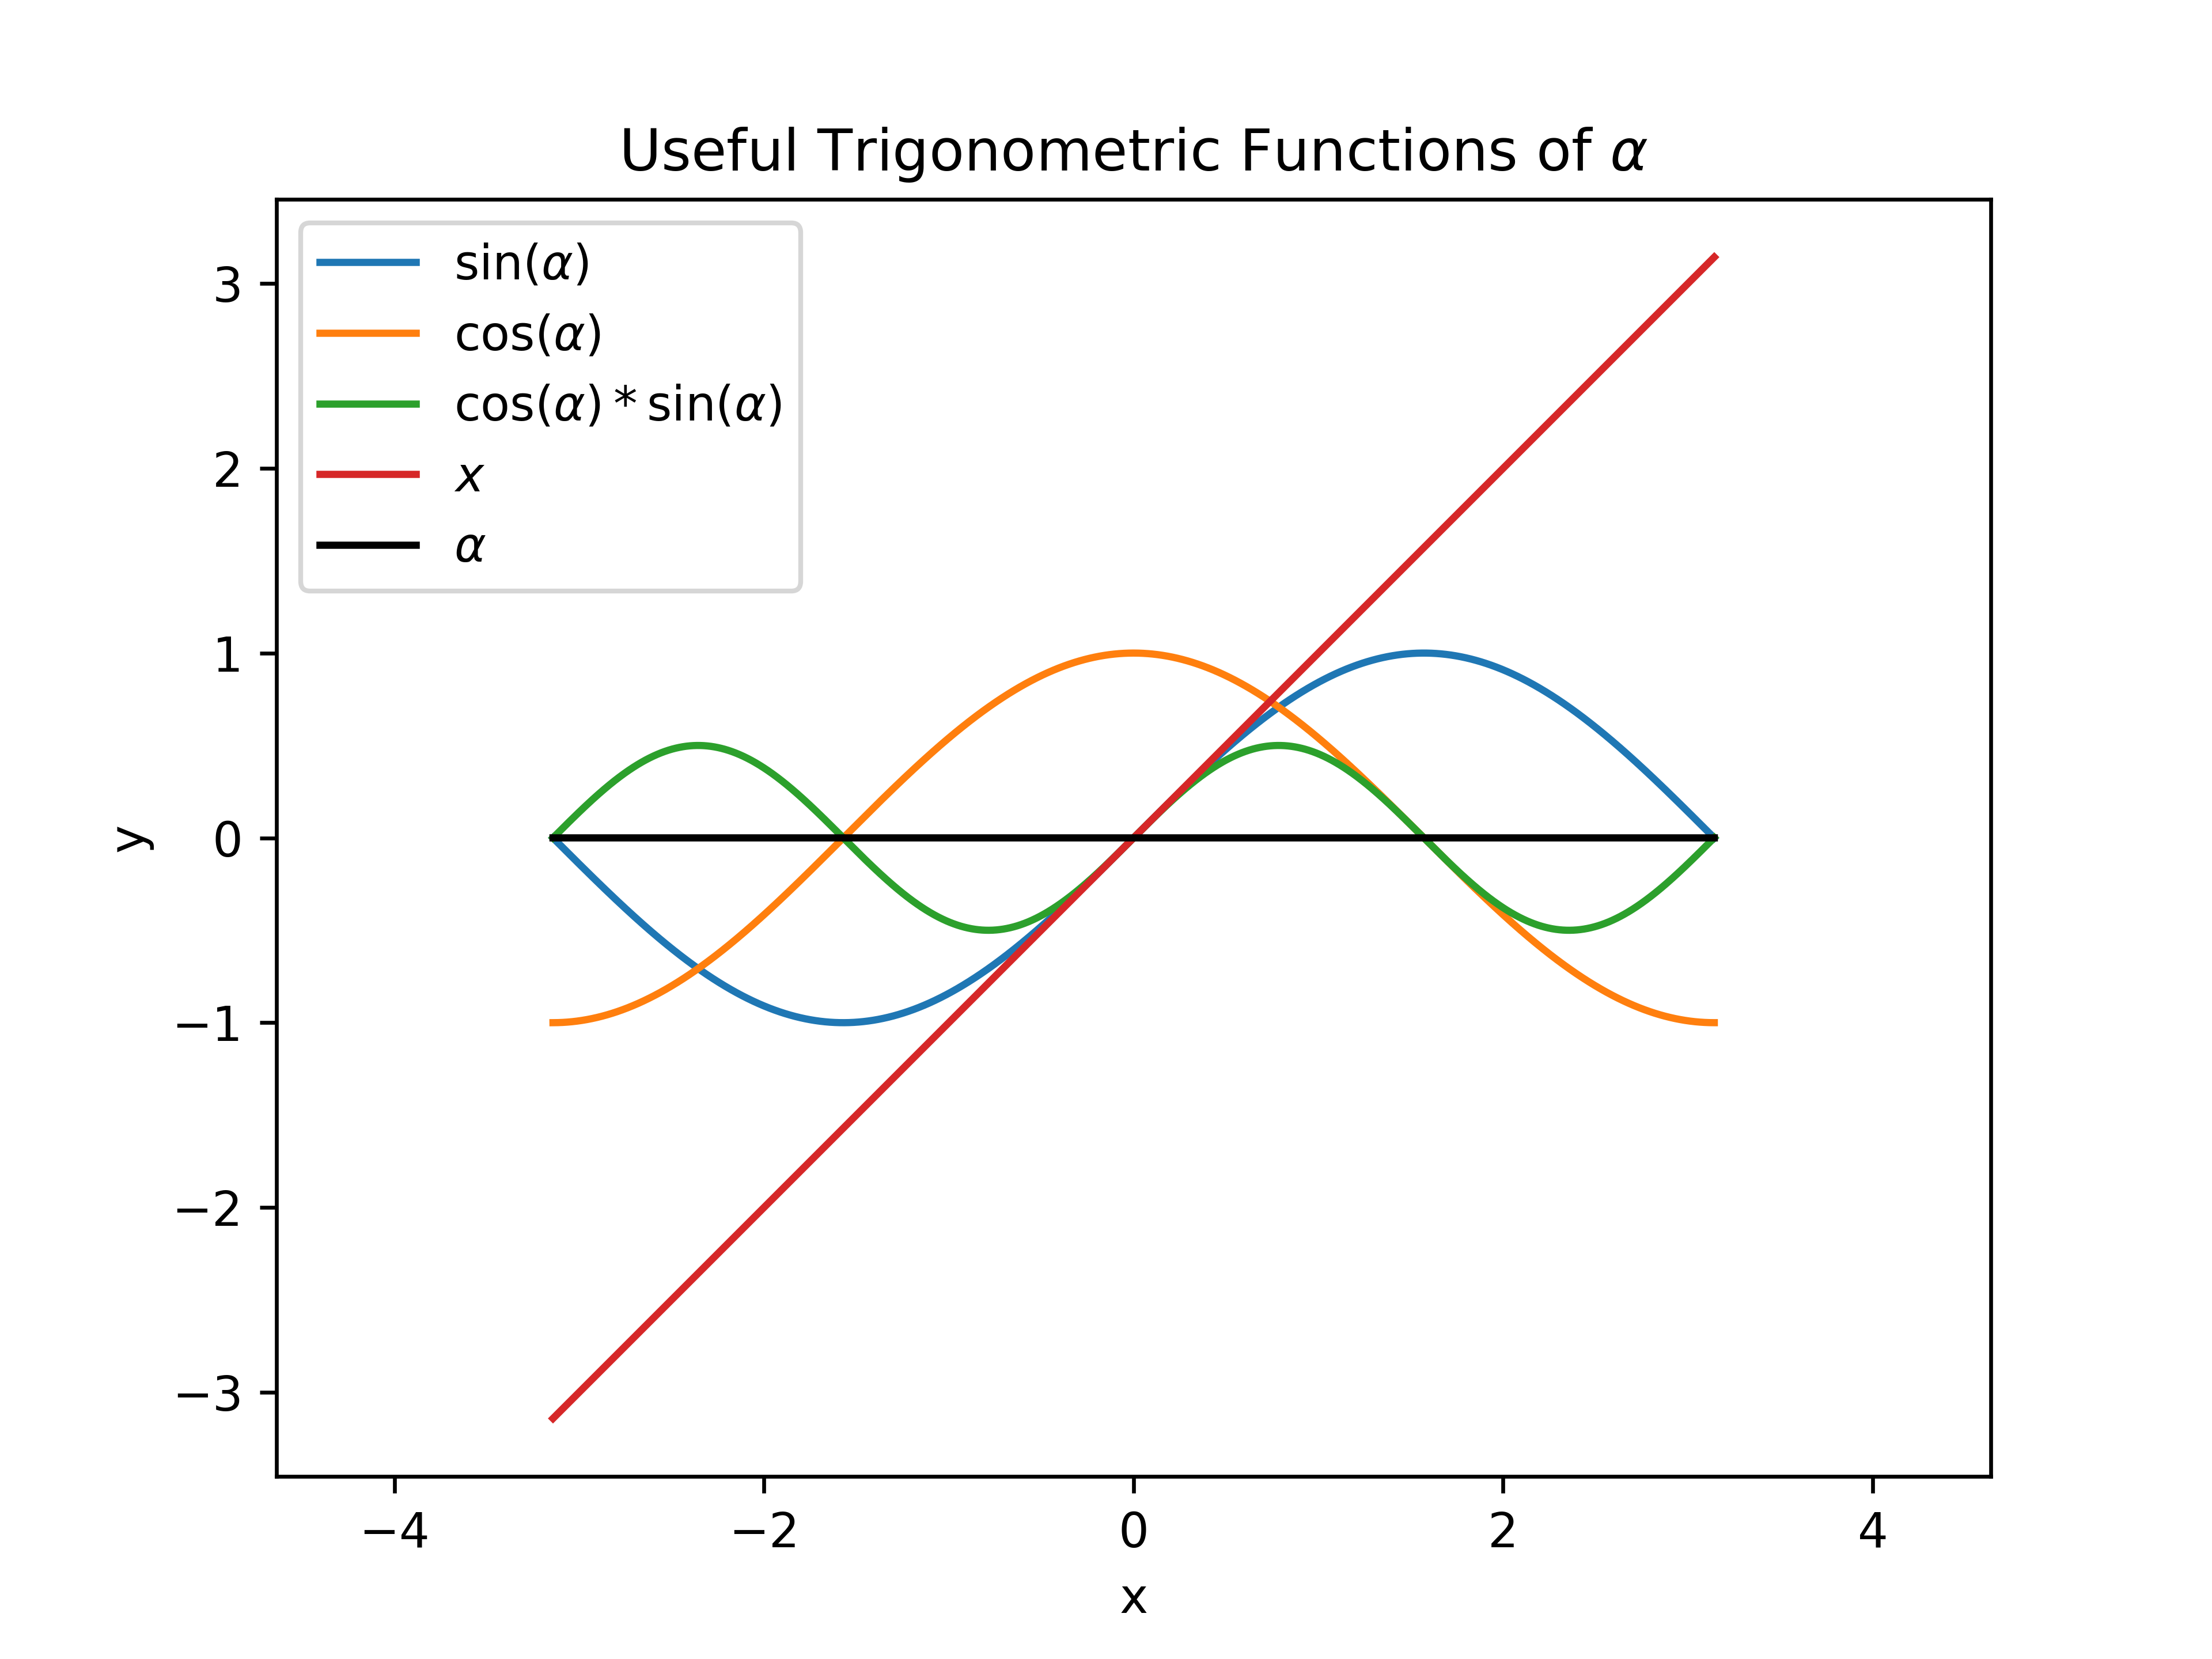
\includegraphics[width=.75\textwidth]{images/plotSinCos}
\caption{Useful Trigonometric Functions of $\alpha$}%
\label{fig:plotSinCos}
\end{figure}

This shows that, in the neighborhood of $\alpha=0$, the distance error $e$ converges linearly at a rate of $-\gamma$.
The angle errors converge at a rate of $-\sigma$, where $-\sigma$ is the real part of the dominant pole of the linear system $A$ in (\ref{eq:lyapunovLinearSystem}).
The poles of the system are the eigenvalues of $A$.
The reason that the errors converge at those rates is that, for the distance error, $e=\text{exp}(-\gamma t)$ is a solution to the equation $\dot{e}=-\gamma e$ since 
\begin{align*}
\tfrac{d}{dt}e=\tfrac{d}{dt}\text{exp}(-\gamma t) = -\gamma \text{exp}(-\gamma t)=-\gamma e.
\end{align*}
Similarly, the behavior of the angle errors is related to the matrix $A$.
Nonsingular matrices can be factored into the form $A=S\Lambda S^{-1}$, where $S$ contains the eigenvectors of $A$ and $\Lambda$ is a diagonal matrix containing the eigenvalues of $A$.
The solution to the differential equation is
\begin{align*}
\left[\begin{array}{c} \dot{\alpha} \\ \dot{\theta} \end{array}\right] = \text{exp} (At)=\text{exp} (S\Lambda~S^{-1}t)=S\text{exp} (\Lambda~t) S^{-1}
\end{align*}
and $\dot{\alpha}$ has the solution $\alpha=\text{exp}(\lambda_\alpha t)$, while $\dot{\theta}$ has the solution $\theta=\text{exp}(\lambda_\theta t)$.

In parking mode, three reasonable design considerations in selecting the gains are:
\begin{itemize}
\item limit the maximum linear velocity,
\item find critically damped gains,
\item have angle errors converge before distance error.
\end{itemize}
Limiting the maximum linear velocity has been discussed already and involves the selection of $\gamma$.
The damping of the system $A$ is determined by
\begin{align*}
\zeta = \frac{\lambda_\alpha(A)}{\lambda_\theta(A)}
\end{align*}
and the gains are critically damped when $\zeta = 1 \Rightarrow \lambda_\alpha(A)=\lambda_\theta(A)=\lambda$.
This causes both angle errors, $\alpha$ and $\theta$, to converge to zero at the same rate.
When the system is critically damped the angle errors will converge faster than the distance error if $\sigma>\gamma$, since that means the rate of convergence for the angle errors is greater than the rate of convergence for the distance error.
In the case where the $A$ matrix is overdamped $\zeta > 1 \Rightarrow \lambda_\alpha(A) > \lambda_\theta(A)$, $\alpha$ will converge to zero faster than $\theta$.
Conversely, when $A$ is underdamped, $\zeta < 1$ and $\theta$ converges faster than $\alpha$.

By selecting the gains to satisfy the design considerations above, the robot will align itself with the goal heading before arriving at the goal point.
The result is that the robot will smoothly decrease its linear velocity as it approaches the goal point.
One alternative occurs when the distance error converges faster than the angle errors, $\gamma>\sigma$, and the robot will get to the goal point and then finish aligning with the goal heading.
In parking mode this leads to several problems: (i) the robot does not look as intelligent since the trajectory does not appear to be as ``natural'' as the way a human would drive; and (ii) rotating in place is typically a much more difficult maneuver for tracked robots to perform and increases fatigue on the treads compared to turning while driving forward.
In driving mode, the case when $\gamma>\sigma$ is not such a problem, because the linear velocity is kept large enough that the robot does not slow down as often.

To deterministically discover gains that will satisfy the properties discussed for parking mode, two conditions must be met:
\begin{itemize}
\item $\zeta = 1$
\item $\sigma > \gamma$
\end{itemize}
For $\zeta=1$, it is necessary to first determine the eigenvalues of $A$.
\begin{align*}
&\text{det}(A-\lambda I) = \left|\begin{array}{c c} -k-\lambda & -h\gamma \\ \gamma & -\lambda\end{array}\right| = 0 \\
\Rightarrow~& (-k-\lambda) (-\lambda)+h\gamma^2 = 0 \\
\Rightarrow~&\lambda^2 + k\lambda+h\gamma^2 = 0 \\
\Rightarrow~&\lambda= \frac{-k\pm\sqrt{k^2-4h\gamma^2}}{2}% chktex 8
\end{align*}
For $\lambda_\alpha(A)=\lambda_\theta(A)$, the term inside the square root must be equal to zero resulting in
\begin{align*}
&k^2 - 4h\gamma^2 = 0 \\
\Rightarrow &k = \sqrt{4h\gamma^2} = 2\gamma\sqrt{h}.
\end{align*}
To find $\sigma>\gamma$ constrained by $k=2\gamma\sqrt{h}$ it is necessary to have
\begin{align*}
\sigma &= -\lambda = \tfrac{k}{2} > \gamma \\
\Rightarrow k &> 2\gamma
\end{align*}
The two equations can be combined to find $h$ such that
\begin{align*}
k &= 2\gamma\sqrt{h} > 2\gamma \\
\Rightarrow h &> 1
\end{align*}

Using this method, any two gains can be selected and the third gain can be found which satisfies the above properties.
For example, setting $\gamma=0.25$ to limit the maximum linear velocity and $h=1.1$ to keep it small but greater than $1$ leads to $k=2\gamma\sqrt{h}=0.52$.
From this it can be seen that $\lambda_\alpha(A) = \lambda_\theta(A) = 0.26 \Rightarrow \zeta = 1$, so the system $A$ is critically damped and $\sigma = 0.26>0.25=\gamma$, causing the angle errors to converge faster than the distance error.

When using (\ref{eq:moveTargetFrame}) to move the goal frame and put the robot into driving mode, it may be more desirable to generate trajectories such that the robot stays on a straight line path to the next waypoint.
The result is that the angle errors are decreased and the robot drives faster as it goes through intermediate waypoints.
One way to have the robot drive towards the waypoint is to set the gains such that the distance error converges faster than the angle errors, and have $\alpha$ converge faster than $\theta$.
An example of the gains that produce these effects is $\gamma=0.25$, $h=0.33$ and $k=0.30$.
Another way to cause the robot to drive on the line segment connecting the previous and current waypoints is to set the target heading to be the angle from the previous waypoint to the current waypoint.

The model-based controller developed in this chapter, along with the analysis of selecting appropriate gains, replaces the original PID controller when answering the question ``How do I get there?''.
